% Options for packages loaded elsewhere
\PassOptionsToPackage{unicode}{hyperref}
\PassOptionsToPackage{hyphens}{url}
%
\documentclass[
]{article}
\usepackage{lmodern}
\usepackage{amssymb,amsmath}
\usepackage{ifxetex,ifluatex}
\ifnum 0\ifxetex 1\fi\ifluatex 1\fi=0 % if pdftex
  \usepackage[T1]{fontenc}
  \usepackage[utf8]{inputenc}
  \usepackage{textcomp} % provide euro and other symbols
\else % if luatex or xetex
  \usepackage{unicode-math}
  \defaultfontfeatures{Scale=MatchLowercase}
  \defaultfontfeatures[\rmfamily]{Ligatures=TeX,Scale=1}
\fi
% Use upquote if available, for straight quotes in verbatim environments
\IfFileExists{upquote.sty}{\usepackage{upquote}}{}
\IfFileExists{microtype.sty}{% use microtype if available
  \usepackage[]{microtype}
  \UseMicrotypeSet[protrusion]{basicmath} % disable protrusion for tt fonts
}{}
\makeatletter
\@ifundefined{KOMAClassName}{% if non-KOMA class
  \IfFileExists{parskip.sty}{%
    \usepackage{parskip}
  }{% else
    \setlength{\parindent}{0pt}
    \setlength{\parskip}{6pt plus 2pt minus 1pt}}
}{% if KOMA class
  \KOMAoptions{parskip=half}}
\makeatother
\usepackage{xcolor}
\IfFileExists{xurl.sty}{\usepackage{xurl}}{} % add URL line breaks if available
\IfFileExists{bookmark.sty}{\usepackage{bookmark}}{\usepackage{hyperref}}
\hypersetup{
  hidelinks,
  pdfcreator={LaTeX via pandoc}}
\urlstyle{same} % disable monospaced font for URLs
\usepackage{longtable,booktabs}
% Correct order of tables after \paragraph or \subparagraph
\usepackage{etoolbox}
\makeatletter
\patchcmd\longtable{\par}{\if@noskipsec\mbox{}\fi\par}{}{}
\makeatother
% Allow footnotes in longtable head/foot
\IfFileExists{footnotehyper.sty}{\usepackage{footnotehyper}}{\usepackage{footnote}}
\makesavenoteenv{longtable}
\usepackage{graphicx}
\makeatletter
\def\maxwidth{\ifdim\Gin@nat@width>\linewidth\linewidth\else\Gin@nat@width\fi}
\def\maxheight{\ifdim\Gin@nat@height>\textheight\textheight\else\Gin@nat@height\fi}
\makeatother
% Scale images if necessary, so that they will not overflow the page
% margins by default, and it is still possible to overwrite the defaults
% using explicit options in \includegraphics[width, height, ...]{}
\setkeys{Gin}{width=\maxwidth,height=\maxheight,keepaspectratio}
% Set default figure placement to htbp
\makeatletter
\def\fps@figure{htbp}
\makeatother
\setlength{\emergencystretch}{3em} % prevent overfull lines
\providecommand{\tightlist}{%
  \setlength{\itemsep}{0pt}\setlength{\parskip}{0pt}}
\setcounter{secnumdepth}{-\maxdimen} % remove section numbering

\author{}
\date{}

\begin{document}

\hypertarget{introduction-to-asipmeister}{%
\section{Introduction to
ASIPMeister}\label{introduction-to-asipmeister}}

\textbf{{1 Week}}

\textbf{Motivation and introduction}

In this exercise, you will be introduced to \emph{ASIP Meister} and our
special directory structure. The overall workflow of the tools is given
at the end; you do not need to deeply look into this. It is just an
overview; we will learn gradually about this flow. First, to understand
the directory structure, you have to read Chapter~2.4 from the
Laboratory Script. Then you will create your first \emph{ASIP Meister}
project and you will go through the \emph{ASIP Meister} ``\emph{User
Manual}'' and ``\emph{Tutorial}'' to get used to \emph{ASIP Meister}.
Afterwards you will simulate a given Assembly Code with \emph{dlxsim}.
Therefore, you will have to read the Chapters~2.3 of the Laboratory
Script. For every part, that starts like ``a)'', ``b)'' \ldots{} you
have to mail the answers and asked files to
\textbf{sajjad.hussain@kit.edu} and use the topic ``asipXX-Session2'',
with XX replaced by your group number.

\textbf{Exercises}

\begin{enumerate}
\def\labelenumi{\arabic{enumi}.}
\item
  \textbf{Preparing the Lab tools environment}

  \begin{enumerate}
  \def\labelenumii{\arabic{enumii}.}
  \item
    ASIPmeister is only installed on i80pc57. It is preferred that you
    always SSH to this PC.
  \item
    Use the public-key authentication system discussed in Chapter 2.2.1
    of the Laboratory Script to avoid typing your password each time
    when logging into frequently.
  \item
    To start, ASIPmeister, ModelSim \& Xilinx ISE during the lab, you
    need to export the following variables each time, or you can add it
    in your ``\emph{/home/.bashrc.user}'' to load automatically when you
    start shell terminal.
  \end{enumerate}
\end{enumerate}

\begin{quote}
export ASIPS\_LICENSE=29000@i80asip.ira.uka.de

export PATH=/AM/ASIPmeister/bin:\$PATH

export ASIP\_APDEV\_SRCROOT=/home/asip00/epp/AM\_tools ***

export PATH=/usr/java/jre1.6.0\_45/bin:\$PATH

export ASIPmeister\_Home=/AM/ASIPmeister

export ASIPmeister\_HOME=/AM/ASIPmeister

source /home/adm/modelsim\_66d.setup

source /home/adm/xilinx\_13.2\_32bit.setup
\end{quote}

\begin{enumerate}
\def\labelenumi{\arabic{enumi}.}
\setcounter{enumi}{3}
\item
  Copy ``\emph{AM\_tools}'' from ``\emph{asip00/epp}'' directory to your
  account, for example at your home folder. Export different
  environmental variables for ASIPmeister and ModelSim or put them in
  the \emph{\textbf{bashrc.user}} and set ``\emph{AM\_tools}'' path from
  your home folder. It needs write permissions.
\end{enumerate}

*** If the ASIPmeister gives error ``could not the old work directory
for binutils''. Copy ``AM\_tools'' to your home directory and set the
path accordingly.

\begin{enumerate}
\def\labelenumi{\arabic{enumi}.}
\setcounter{enumi}{1}
\item
  \textbf{Preparing your project}

  \begin{enumerate}
  \def\labelenumii{\arabic{enumii}.}
  \item
    Create a project directory for this session by copying the directory
    ``\emph{/home/asip00/­epp/ /TEMPLATE\_PROJECT/}'' and renaming it
    (e.g. \emph{brownie}).
  \item
    For each application (C or Assembly), you have to create a separate
    subdirectory in the ``\emph{Application}'' directory (e.g.
    \emph{LoopExample}).
  \end{enumerate}
\end{enumerate}

\textbf{NOTE: Never name the subdirectory same as the name of the
application that you want to compile using ``\emph{Makefile}''. This
will result in problems for the Makefile script execution.}

\begin{enumerate}
\def\labelenumi{\arabic{enumi}.}
\setcounter{enumi}{2}
\item
  Copy the given assembly file from
  ``/home/asip00/Sessions/Sessions/Session1/'' into this application
  subdirectory i.e. \emph{LoopExample}.
\item
  Copy a ``\emph{Makefile}'' file from the ``\emph{TestPrint}''
  application subdirectory to each application subdirectory. This
  Makefile has been prepared to help you in performing different tasks
  during the Lab as discussed in Figure 2-3 in the Laboratory Script.
\item
  In an application directory, typing, ``\emph{make help}'' on shell
  terminal will show usage of the ``\emph{Makefile}'' and how different
  parameters can be passed.
\item
  Copy the provided \emph{ASIPMeister} CPU file ``\emph{browstd32.pdb''}
  from ``/home/asip00//Sessions/Session1/'' into your project directory.
\item
  Set proper parameters and settings in ``\emph{env\_settings}'' as
  discussed in Figure 2-5 in the Laboratory Script. Specially the
  followings:
\end{enumerate}

\begin{quote}
export PROJECT\_NAME=brownie

export CPU\_NAME=browstd32

export ASIPMEISTER\_PROJECTS\_DIR=\$\{HOME\}/ASIPMeisterProjects

export DLXSIM\_DIR=/home/asip00/epp/dlxsimbr\_Laboratory
\end{quote}

\begin{enumerate}
\def\labelenumi{\arabic{enumi}.}
\setcounter{enumi}{7}
\item
  Using above steps, for each session, you need to create a separate
  project if you have modified the CPU or you can have separate
  application subdirectories for the same CPU.
\end{enumerate}

\begin{enumerate}
\def\labelenumi{\arabic{enumi}.}
\setcounter{enumi}{2}
\item
  \textbf{Using ASIP Meister}

  \begin{enumerate}
  \def\labelenumii{\arabic{enumii}.}
  \item
    In your project directory, start \emph{ASIPMeister} for the given
    basis CPU: ``\emph{ASIPmeister browstd32.pdb \&}''. Moreover, do not
    forget to start \emph{ASIP Meister} in your project directory,
    because it will create the ``\emph{meister''} subdirectory to
    generate different VHDL files and GNU tools, where it is started.
    The ``\emph{meister''} subdirectory is expected to be in your
    current project directory.
  \item
    Read the \emph{ASIP Meister} ``\emph{User Manual}'' and
    ``\emph{Tutorial}'' to get used to the GUI. You can find the related
    files in the ``\emph{/home/asip00/Documents}'' \emph{directory}.
    Read systematically through both files simultaneously and play with
    the specific parts of the GUI for which you are currently reading
    the user manual and tutorial.
  \item
    If you anyhow configure something wrong, then just reload the
    original file. The most important parts for the later work are the
    ``\emph{Resource Declaration}'', ``\emph{Instruction Definition}'',
    ``\emph{MicroOp Description}'', ``\emph{HDL Generation}'', ``\emph{C
    Definition}'' and ``\emph{Compiler Generation}'' so have a detailed
    look at them.
  \item
    Go through all the steps one-by-one as mentioned in the tutorial and
    generate VHDL files and GNU Tools. VHDL files will later be used in
    ModelSim for hardware simulation, while GNU tools will be used to
    compile, assemble, and link your application code. In this step,
    recommended settings are "\emph{VHDL}" and "\emph{sim. model and
    syn. model}".
  \item
    Make sure that AM\_tools path is set properly in your
    ``bashrc.user'' and is permissible.
  \item
    Make sure that you complete both/two steps i.e. "\emph{Input
    Description Generation}" and "\emph{GNU Tools Generation}".
  \item
    GNU Tool generation may take 10-15minutes. After GNU Tool
    generation, you will see compiler, assemble and linker according to
    your instruction sets. See the directory in
    \$\{ASIPMEISTER\_PROJECTS\_DIR\}/\$\{PROJECT\_NAME\}/meister/\$\{CPU\_NAME\}.
    swgen/bin.
  \end{enumerate}
\end{enumerate}

\begin{enumerate}
\def\labelenumi{\alph{enumi})}
\item
  How many pipeline-stages this CPU has? Normally, CPU has fetch,
  decode, execute, memory and write-back stages, how these stages are
  mapped into brownie 4 stage CPU? For CPU related details look at the
  Brownie32-Std datasheet at /home/asip00/epp/Documents.
\end{enumerate}

\begin{quote}
\textbf{Resource Declarations:}
\end{quote}

\begin{enumerate}
\def\labelenumi{\alph{enumi})}
\setcounter{enumi}{1}
\item
  See different hardware resources used in the CPU. Select ALU in the
  "Instance" list. What do you understand from the contents of "Function
  Set" tab? What is listed there?
\item
  How many does read/write ports GPR has?
\item
  CPU uses full forwarding in pipeline. How many forwarding units are
  used? How many intermediate register values can we forward now?
\item
  What should we need to change in GPR and Forwarding Units if we need
  an instruction, which writes two operands like quotient and remainder
  (DIV rd1, rd2, rs1, rs2) to be returned?
\end{enumerate}

\begin{quote}
\textbf{Storage Spec:}
\end{quote}

\begin{enumerate}
\def\labelenumi{\alph{enumi})}
\setcounter{enumi}{5}
\item
  What does GPR0-7 are used for?
\end{enumerate}

\begin{quote}
\textbf{Instruction Definition:}
\end{quote}

\begin{enumerate}
\def\labelenumi{\alph{enumi})}
\setcounter{enumi}{6}
\item
  Why does this CPU have \textbf{SP} instruction format? What
  instructions are covered by this \textbf{SP} format? Can we map these
  instructions with some other format and remove SP format from the CPU?
\end{enumerate}

\begin{quote}
\textbf{Micro Op. Description:}
\end{quote}

\begin{enumerate}
\def\labelenumi{\alph{enumi})}
\setcounter{enumi}{7}
\item
  What does ForwardDataFromWB() and ForwardDataFromEXE() are doing?
  Which hardware resources are being used here?
\item
  What does GPRRead(src1) macro perform? Why FWO.forward() is used here?
\item
  What does ``\emph{alu\_flag}'' mean in ALUExec() macro? What does
  individual bits mean?
\end{enumerate}

\begin{quote}
\textbf{VHDL Generation:}
\end{quote}

\begin{enumerate}
\def\labelenumi{\alph{enumi})}
\setcounter{enumi}{10}
\item
  What does different bits in ``\emph{alu\_flag}'' stand for? You can
  take help from the generated VHDL for understanding
  ``\emph{alu\_flag}'' in fhm\_alu\_w32.vhd.
\end{enumerate}

\begin{enumerate}
\def\labelenumi{\arabic{enumi}.}
\setcounter{enumi}{3}
\item
  \textbf{Simulating with dlxsim}

  \begin{enumerate}
  \def\labelenumii{\arabic{enumii}.}
  \item
    Now you have a CPU that is able to execute the given example code
    \emph{6\_for.s}. This code has implemented the following part:
  \end{enumerate}
\end{enumerate}

\begin{quote}
for (i=0; i\textless10; i++) \{

A{[}i{]} = B{[}i{]} + 5 + C;

\}
\end{quote}

\begin{enumerate}
\def\labelenumi{\arabic{enumi}.}
\setcounter{enumi}{1}
\item
  In this session, we only simulate the assembly code with
  \emph{dlxsim}. You should have a copy for the ``\emph{Makefile}'' in
  your ``\emph{LoopExample}'' subdirectory.
\item
  Then, go to the ``\emph{LoopExample}'' subdirectory inside your
  Applications directory and execute ``\emph{make sim}''.
\item
  When ``\emph{make sim}'' is finished, a new subdirectory called
  ``\emph{BUILD\_SIM}'' containing some important files is created in
  your current directory. There is a special ``\emph{.\textbf{dlxsim}}''
  file used for dlxsim simulation and there are ``\emph{TestData.IM}''
  and ``\emph{TestData.DM}'' files used for ModelSim simulation.
  \emph{TestData.IM} and \emph{TestData.DM} are instruction and data
  memory image files respectively.
\item
  Simulate ``\emph{.dlxsim}'' file with dlxsim by typing: ``\emph{make
  dlxsim}'' with default settings or ``\emph{make dlxsim
  DLXSIM\_PARAM="-fBUILD\_SIM/LoopExample.dlxsim -da0 --pf1}". The
  parameter pf1 indicates the full forwarding in CPU pipeline, for
  details see brownie32-std datasheet.
\item
  Inside dlxsim terminal, you can use ``go'' to execute whole program,
  ``step'' to execute one instruction at a time, and ``stats'' to see
  the statistics.
\item
  The command ``make sim'' adds some start-up and ending code to your
  program to generate a ``.dlxsim'' file which is then executed by
  ``make dlxsim''. You can directly run your assembly program only using
  dlxsim like DLXSIM\_PATH/dlxsim --f\textbf{Assembly.s} --da0 --pf1
\end{enumerate}

\begin{enumerate}
\def\labelenumi{\alph{enumi})}
\item
  What is meant by the following lines and values in the dlxsim:
\end{enumerate}

\begin{quote}
Biggest used address for Text Section (word aligned): 0xdc

Biggest used address for Data Section (word aligned): 0x130
\end{quote}

\begin{enumerate}
\def\labelenumi{\alph{enumi})}
\setcounter{enumi}{1}
\item
  In Dlxsim, you can use "\emph{get start\_address
  \#of\_of\_instructions}" to see the 32-bit binary values of each
  instructions and from this, you can also extract opcodes. As ``get \_A
  10d'' will show 10 values for array A in decimal. What does ``get 0
  10'' gives you? What are these values?
\item
  Can you see the data \_A, \_B and \_C variables in TestData.DM? What
  does the first 32-bit word indicate? This large value is a stack
  pointer value, used while you call many subroutines one by one. Why
  this value is so large?
\item
  How many cycles are required to execute this program?
\end{enumerate}

\begin{quote}
\textbf{Next Session:} Assembly Programs

\textbf{Readings for the next session}: Laboratory Chapters 8.1, 8.2,
8.3

BrownieSTD32 Datasheet Introduction and Section 1.1 - 1.3

2.2.3. Instruction Set Quick Reference

4. Memory Access

Appendix A. Delayed Load
\end{quote}
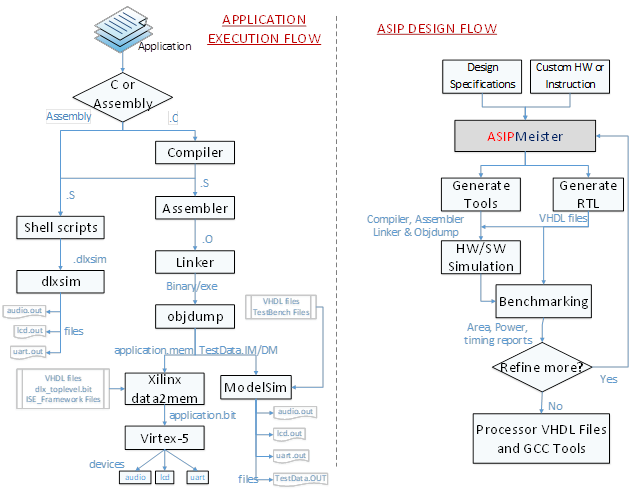
\includegraphics[width=5.65694in,height=4.08958in]{1.png}
Figure 1: An overview of our Lab Tools

\hypertarget{assembly-programs}{%
\section{\texorpdfstring{Assembly
\textbf{Programs}}{Assembly Programs}}\label{assembly-programs}}

\textbf{{1 Week}}

\textbf{Motivation and Introduction}

The main goal of this session is to get used to assembly programs. Every
example shows a basic operation. Examine the code, simulate it with
\emph{dlxsim} and answer the corresponding questions. The assembly code
is available in the directory
``\emph{/home/asip00/Sessions/Session2/''}. \emph{Dlxsim} is available
in the directory
``\emph{asip00/}\emph{epp/dlxsimbr\_}\emph{Laboratory/'' (default)}. You
can copy \emph{dlxsim} to your directory or you can start it from the
default directory. For every exercise, the part that starts like ``a)'',
``b)'' \ldots{} you have to write an answer. This answer should mainly
prove that you have understood the problem, so you can make your answers
short, but they still have to answer everything, that was asked. Mail
your answer to \textbf{sajjad.hussain@kit.edu} and use the topic
``asipXX-Session1'', with XX replaced by your group number.

\textbf{Exercises}

The following exercise correspond to the given assembly files in the
``\emph{/home/asip00/Sessions/Session1}'' directory.

\begin{enumerate}
\def\labelenumi{\arabic{enumi}.}
\item
  \textbf{Preparing your project}

  \begin{enumerate}
  \def\labelenumii{\arabic{enumii}.}
  \item
    You can use the same project as in the last session, and just create
    a separate application subdirectory for each assembly example. You
    can start a fresh project as in the Session 1, but this would be
    time consuming.
  \item
    For each application (C or Assembly), you have to create
    subdirectories in the ``\emph{Application}'' directory.
  \item
    Copy a ``\emph{Makefile}'' file from the ``\emph{TestPrint}''
    subdirectory to each application subdirectory.
  \item
    Set proper parameters and settings in ``\emph{env\_settings}.
  \item
    For these exercises, we will run basic assembly programs in dlxsim
    and see the effect of pipeline forwarding (-pf1) or no forwarding
    (-pf0), like
  \end{enumerate}
\end{enumerate}

\begin{quote}
\emph{make dlxsim DLXSIM\_PARAM="-da0 -pf0}"
\end{quote}

\begin{enumerate}
\def\labelenumi{\arabic{enumi}.}
\setcounter{enumi}{1}
\item
  \textbf{Basic Assembly Instructions}
\end{enumerate}

Understand the functionality of every instruction and understand the
values of every target register after the program run has completed (see
the dlxsim chapter for reading register values in dlxsim simulation).
Check the number of cycles needed to execute all instructions.

\begin{enumerate}
\def\labelenumi{\alph{enumi})}
\item
  What is the reason for this high number of cycles? Which instruction
  causes that behaviour and why is it doing so?
\item
  What is the code/data address space? What is starting and ending
  address of code/data section?
\end{enumerate}

\begin{enumerate}
\def\labelenumi{\arabic{enumi}.}
\setcounter{enumi}{2}
\item
  \textbf{Memory Access}
\end{enumerate}

\begin{enumerate}
\def\labelenumi{\alph{enumi})}
\item
  Explain the goal of the instruction combination \emph{LSOI /ADDI}.
  What is generally (so: not only for this specific example) the
  register value after \emph{ADDI}, what is it after the additional
  \emph{LSOI}?
\item
  Why is it in general not possible to omit the \emph{LSOI} instruction,
  although it would be possible in this special example?
\item
  Read about ``forwarding'' and ``load delay slot'' in brownie32
  datasheet. Disable NOP after the load instruction, and try executing
  with --pf0 and --pf1 both.
\end{enumerate}

\begin{enumerate}
\def\labelenumi{\arabic{enumi}.}
\setcounter{enumi}{3}
\item
  \textbf{Branches}
\end{enumerate}

\begin{enumerate}
\def\labelenumi{\alph{enumi})}
\item
  Which high-level control structure (e.g. `call subroutine' \ldots) is
  implemented in this example code?
\item
  What is computed with this example? R24 = \emph{function} (R21, R22);
\item
  Look at the \emph{NOP} instructions and explain why they are placed
  there.
\end{enumerate}

\begin{enumerate}
\def\labelenumi{\arabic{enumi}.}
\setcounter{enumi}{4}
\item
  \textbf{Loops}
\end{enumerate}

\begin{enumerate}
\def\labelenumi{\alph{enumi})}
\item
  What is computed with this example? R23 = \emph{function} (R21, R22).
  Debug the application step-by-step with the capabilities of dlxsim.
\item
  The approach to compute the function in the way this example is doing
  it has two specific names. Do you know those names? (One is founded by
  the main operations, while the other is founded historically. You
  either know the names or you don't. If you don't know both names, you
  may guess)
\item
  In general, how often is the loop maximally executed? How the input
  data has to look like to get this maximal number of iterations?
\item
  Enable and disable the first NOP, and try executing with --pf0 and
  --pf1 both.
\end{enumerate}

\begin{enumerate}
\def\labelenumi{\arabic{enumi}.}
\setcounter{enumi}{5}
\item
  \textbf{A High Level Structure}
\end{enumerate}

\begin{enumerate}
\def\labelenumi{\alph{enumi})}
\item
  Which high-level control structure do you recognize? Explain the
  purpose of the instruction-block between ``\emph{ADDI R23, R0,
  \$(2)}'' and ``\emph{JPR R24}''.
\item
  Why do you have to shift by value 3? Explain it with a close view to
  the body of the control structure and pay attention to the addressing
  mode of the DLX processor.
\item
  What are the general differences between branch and jump instructions
  in the DLX instruction set (also have a look at the different
  instruction formats to find a part of the answer)?
\end{enumerate}

\begin{enumerate}
\def\labelenumi{\arabic{enumi}.}
\setcounter{enumi}{6}
\item
  \textbf{ASM Directive in C}

  \begin{enumerate}
  \def\labelenumii{\arabic{enumii}.}
  \item
    You can use assemble instruction directly in c as follows {[}1,2{]}:
  \end{enumerate}
\end{enumerate}

\begin{quote}
int res=0;

int in1=20;

int in2=30;

int main() \{

\textbf{\_\_asm\_\_ volatile (}

"add \%{[}out{]}, \%{[}op1{]}, \%{[}op2{]}\textbackslash n"

: {[}out{]} "=\&r" (res)

: {[}op1{]} "r" (in1),{[}op2{]} "r" (in2)

);

return 0;

\}
\end{quote}

\begin{enumerate}
\def\labelenumi{\arabic{enumi}.}
\setcounter{enumi}{1}
\item
  In any asm block, assembly instructions appear first, followed by the
  inputs and outputs, which are separated by a colon. The assembly
  instructions can consist of one or more quoted strings. The first
  colon separates the output operands; the second colon separates the
  input operands. If there are clobbered registers, they are inserted
  after the third colon. If there are no clobbered inputs for the asm
  block, the third colon can be omitted, as Listing 2 shows.
\end{enumerate}

\begin{quote}
int A{[}10{]} = \{45,23,0,0,0,0,0,0,0,0\};

int main() \{

\textbf{\_\_asm\_\_volatile (}

"add \%{[}out{]}, \%{[}op1{]}, \%{[}op2{]} \textbackslash n"

: {[}out{]} "=\&r" (A{[}2{]})

: {[}op1{]} "r" (A{[}0{]}), {[}op2{]} "r" (A{[}1{]})

);

return 0;

\}
\end{quote}

\begin{enumerate}
\def\labelenumi{\arabic{enumi}.}
\setcounter{enumi}{2}
\item
  There is no output operand for the sw instruction, hence the outputs
  section of the asm is empty. None of the registers is modified, so
  they are all input operands, and the target address is passed in with
  the input operands. However, something is modified: the addressed
  memory location.
\end{enumerate}

\begin{quote}
int res {[}{]} = \{0,0,0,0,0,0,0,0\};

int a=45;

int main() \{

\textbf{\_\_asm\_\_ volatile (}

" sw \%1(\%2), \%0 \textbackslash n"

:

: "r"(a), "i"(sizeof(int)),"r"(\&res)

);

return 0;

\}
\end{quote}

\begin{enumerate}
\def\labelenumi{\arabic{enumi}.}
\setcounter{enumi}{3}
\item
  Branching can be tricky with inline asm. Using labels, the branch-to
  address can be designated with a unique identifier that can be used as
  a target branch address.
\end{enumerate}

\begin{quote}
int x, y, z;

int a=45, b=23, c=1;

int main() \{

\_\_asm\_\_ volatile (

" addi \%{[}out1{]}, \%{[}op1{]}, \%{[}op2{]} \textbackslash n"

" brnz \%{[}op3{]}, here \textbackslash n"

" there: add \%{[}out2{]}, \%{[}op1{]}, \%{[}op2{]} \textbackslash n"

" here: mul \%{[}out3{]}, \%{[}op1{]}, \%{[}op2{]} \textbackslash n"

: {[}out1{]} "=\&r" (x), {[}out2{]} "=\&r" (y), {[}out3{]} "=\&r" (z)

: {[}op1{]} "r" (a), {[}op2{]} "r" (b) , {[}op3{]} "r" (c)

: "r0" );

return 0;

\}
\end{quote}

\begin{enumerate}
\def\labelenumi{\arabic{enumi}.}
\setcounter{enumi}{4}
\item
  See ``A guide to inline assembly for C and C++'' for further details.
\end{enumerate}

\begin{enumerate}
\def\labelenumi{\alph{enumi})}
\item
  Write a C program using assembly instructions to load two consecutive
  values from an array and store their addition or subtraction at the
  fourth location of an array depending on the third value of array i.e.
  0 means addition and 1 means subtraction.
\end{enumerate}

\textbf{Next Session:} ModelSim Simulation

\textbf{Readings for the next session}: Chapters 2.3, 4 \& 5

\textbf{{[}1{]}.
\url{https://gcc.gnu.org/onlinedocs/gcc/Extended-Asm.html}}

\textbf{{[}2{]}.\url{https://dmalcolm.fedorapeople.org/gcc/2015-08-31/rst-experiment/how-to-use-inline-assembly-language-in-c-code.html}}

\hypertarget{modelsim-simulation}{%
\section{\texorpdfstring{ModelSim \textbf{Simulation}
}{ModelSim Simulation }}\label{modelsim-simulation}}

\textbf{{1 Week}}

\textbf{Motivation and introduction}

In this session, we will compile a C-code application and simulate the
result in \emph{ModelSim and Dlxsim}. The applications can be assembled
or compiled using a compiler that is already generated by ASIPmeister in
the previous session. ModelSim simulates your code binaries using the
VHDL files generated from the ASIPmeister. While dlxsim only simulates
the instruction one by one and it does not care about the hardware
implementation of the instructions. For every part, that starts like
``a)'', ``b)'' \ldots{} you have to mail the answers and asked
files/tables to \textbf{sajjad.hussain@kit.edu} and use the topic
``asipXX-Session3'', with XX replaced by your group number.

\textbf{Exercises}

\begin{enumerate}
\def\labelenumi{\arabic{enumi}.}
\item
  \textbf{Preparing your project}

  \begin{enumerate}
  \def\labelenumii{\arabic{enumii}.}
  \item
    You can use the same project as in the last session, and just create
    a separate application subdirectory for the application. You can
    start a fresh project as in the Session 1, but this would be time
    consuming.
  \item
    For the C application, you have to create subdirectory in the
    ``\emph{Application}'' directory (e.g. \emph{LoopExampleC}), and
    copy your application from
    ``\emph{/home/asip00/Sessions/Session3/6\_for.c}'' to here.
  \item
    Copy a ``\emph{Makefile}'' file from the ``\emph{TestPrint}''
    application subdirectory to each application subdirectory.
  \item
    Set proper parameters and settings in ``\emph{env\_settings}.
  \item
    For these exercises, we will be using pipeline forwarding (-pf1)
    option which is the default one.
  \item
    Make sure that you already have VHDL files and GNU tools in your
    project's meister directory.
  \end{enumerate}
\item
  \textbf{Compiling and Simulating the Application}

  \begin{enumerate}
  \def\labelenumii{\arabic{enumii}.}
  \item
    Go to your application subdirectory and type ``\emph{\textbf{make
    clean}}'' clean this directory it there are previously generated
    files.
  \item
    Compile the C application using ``\emph{\textbf{make sim}}''. A
    directory ``\emph{\textbf{BUILD\_SIM}}'' is created which contains
    different temporary files and a .dlxsim file to be simulated in
    dlxsim. In this directory, the files ``\emph{\textbf{TestData.IM}}''
    and ``\emph{\textbf{TestData.DM}}''are the file used during the
    ModelSim simulation.
  \item
    In folder BUILD\_SIM, look at the ``\emph{6\_for.s}'' which is
    generated. Another file ``\emph{startup.s}'' is used along with the
    generated ``\emph{6\_for.s}'' to generate TestData.IM/DM files. Just
    understand and remember the structure of ``6\_for.s'' files if you
    have to write your own .s file, and how it is being executed along
    with ``\emph{startup.s}''.
  \item
    Simulate your application in dlxsim simulator using
    ``\emph{\textbf{make dlxsim}}'', just to verify the functionality.
  \item
    In your project directory, go to the ``ModelSim'' directory and
    start the ModelSim using ``\emph{\textbf{vsim}}''
  \item
    If ModelSim asks for ``modelsim.ini'' choose the default one like
    ``/Software/ModelSim/ModelSim\_6.6d/modeltech/modelsim.ini''
  \item
    Open File Menu \textgreater{} New \textgreater{} Project and enter a
    project name (e.g. browstd32) and change the project location to the
    ModelSim directory in your project directory. Confirm the dialog
    with the OK button.
  \item
    Choose ``Add Existing File'' button and browse to the
    meister/dlx\_basis.syn directory of your ASIP Meister project and
    select all the VHDL files for synthesis.
  \item
    Again, choose ``Add Existing File'' button and add the testbench
    files: tb\_browstd32.vhd, MemoryMapperTypes.vhd, MemoryMapper.vhd,
    and Helper.vhd from the ModelSim directory of your current project.
  \item
    {[}Optional{]} Configure the CPU Frequency for which you want to
    simulate your CPU, default is 50 MHz. Open the ModelSim testbench
    (``tb\_ browstd32.vhd''), search for CLK \_PERIOD, and change the
    value accordingly in ``ns''.
  \item
    Compile the project using Compile Menu \textgreater{} Compile Order
    \textgreater{} Auto Generate. Every file should have a green mark
    behind its name, showing that the compilation was successful.
  \item
    Run the simulation using Simulate Menu \textgreater{} Start
    Simulation. Open the work library, mark the entry
    ``\emph{\textbf{cfg}}'' (that is the VHDL configuration for the
    testbench) in the list and press OK. That will start the simulation
    and you will get another two tabs attached to the Workspace window
    (sim / Files).
  \item
    {[}Optional{]} To load some predefined simulation settings choose
    Tools Menu \textgreater{} Tcl \textgreater{} Execute Macro and
    select the ``wave\_vhdl.do'' file in your ModelSim directory and
    press OK to load it. The wave-window is filled with certain signals
    that are useful to evaluate the simulation of the program execution
    on the processor.
  \item
    {[}Optional{]} If you want to dump VCD file of yor design for power
    estimation, you can enter following commands in ModelSim command
    prompt:
  \end{enumerate}
\end{enumerate}

\begin{quote}
VSIM \textgreater{} vsim -t 1ns work.cfg

VSIM \textgreater{} vcd file test.vcd

VSIM \textgreater{} vcd add -r test/dut/*
\end{quote}

\begin{enumerate}
\def\labelenumi{\arabic{enumi}.}
\setcounter{enumi}{14}
\item
  Press the button ``\emph{\textbf{Run all}}'' to run the simulation
  until it aborts. At the end of a simulation the message ``Failure:
  Simulation End'' is printed to show successful end of simulation. At
  the simulation end, the file ``\emph{\textbf{TestData.OUT}}'' is
  created in your ModelSim directory. It contains the content of the
  simulated memory after the CPU finished working. Therefore, if your
  algorithm is storing the result in the memory you can find the values
  here.
\end{enumerate}

\begin{enumerate}
\def\labelenumi{\alph{enumi})}
\item
  How many cycles are required to execute this program DLXsim and
  ModelSim?
\item
  What are the contents of TestData.OUT? Are these correct? First value
  is the stack value; next 10 words belongs to array A, then 10 words
  belongs to array B, and C.
\item
  In the ModelSim waveform window, what is the starting address of PC
  after the reset? Moreover, after how many cycles your
  ``\textbf{main}'' function is started? In the waveform, look at the PC
  and IR values.

  \begin{enumerate}
  \def\labelenumii{\arabic{enumii}.}
  \item
    The default GCC compiler optimization is --O0. Try different
    optimization levels with dlxsim and ModelSim using e.g. ``\emph{make
    dlxsim GCC\_PARAM=-O1}'' or using ``\emph{make sim
    GCC\_PARAM=-O1}''.
  \item
    Repeat this benchmarking for all compiler optimization-levels like
    O0, O1, O2, O3 and O4 for both dlxsim and ModelSim.
  \end{enumerate}
\end{enumerate}

\begin{enumerate}
\def\labelenumi{\alph{enumi})}
\item
  Does the application is executed successfully using different
  optimization levels? If yes, please fill the following benchmark
  table. These optimizations have distinct effects on the size of the
  code.
\end{enumerate}

\begin{longtable}[]{@{}llll@{}}
\toprule
\begin{minipage}[b]{0.22\columnwidth}\raggedright
\textbf{Optimization Level}\strut
\end{minipage} & \begin{minipage}[b]{0.22\columnwidth}\raggedright
\textbf{Executed?}

\textbf{{[}Yes/No{]}}\strut
\end{minipage} & \begin{minipage}[b]{0.22\columnwidth}\raggedright
\textbf{Cycle count\\
}ModelSim\strut
\end{minipage} & \begin{minipage}[b]{0.22\columnwidth}\raggedright
\textbf{Cycle count\\
}dlxsim\strut
\end{minipage}\tabularnewline
\midrule
\endhead
\textbf{-O0 (default)} & & &\tabularnewline
\textbf{-O1} & & &\tabularnewline
\textbf{-O2} & & &\tabularnewline
\textbf{-O3} & & &\tabularnewline
\textbf{-O4} & & &\tabularnewline
\bottomrule
\end{longtable}

\textbf{Next Session:} Synthesis and Hardware Implementation

\textbf{Readings for the next session}: Laboratory Chapters 6

\hypertarget{synthesis-and-hardware-implementation}{%
\section{\texorpdfstring{\textbf{Synthesis and} Hardware
\textbf{Implementation}
}{Synthesis and Hardware Implementation }}\label{synthesis-and-hardware-implementation}}

\textbf{{1 Week}}

\textbf{Motivation and introduction}

In this session we synthesis our basis CPU with Xilinx ISE and execute a
test application on real hardware. The synthesis reports tell us how
much area and power is consumed by our CPU and what is the critical path
of our design. In this session, we will compile a C-code application
direct its output the LCD and UART with the help of some predefined
libraries. This session also introduces about different peripheral where
we forward our text/data, and how different libraries are used for
different peripherals. For every part, that starts like ``a)'', ``b)''
\ldots{} you have to mail the answers and asked files/tables to
\textbf{sajjad.hussain@kit.edu} and use the topic ``asipXX-Session3'',
with XX replaced by your group number.

\textbf{Exercises}

\begin{enumerate}
\def\labelenumi{\arabic{enumi}.}
\item
  \textbf{Preparing your project}

  \begin{enumerate}
  \def\labelenumii{\arabic{enumii}.}
  \item
    You can use the same project as in the last session, and just create
    a separate application subdirectory the application. You can start a
    fresh project as in the Session 1, but this would be time consuming.
  \item
    For the C application, you have to create two subdirectories in the
    ``\emph{Application}'' directory e.g. ``\emph{Hello\_SW}'' and
    ``\emph{Hello\_HW}''. Copy your application from
    ``\emph{/home/asip00/Sessions/Session4/app.c}'' to these. This is a
    simple example to direct a text to some peripheral devices like LCD
    or UART. ``\emph{Hello\_SW}'' is aimed for dlxsim and ModelSim
    simulations and ``\emph{Hello\_HW}'' is aimed for real hardware
    implementation.
  \item
    Copy a ``\emph{Makefile}'' file from the ``\emph{TestPrint}''
    application subdirectory to each application subdirectory.
  \item
    Set proper parameters and settings in ``\emph{env\_settings}.
  \item
    For these exercises, we will be using pipeline forwarding (-pf1)
    option which is the default one.
  \item
    Make sure that you already have VHDL files and GNU tools in your
    project's meister directory.
  \end{enumerate}
\item
  \textbf{Compiling and ModelSim Simulation}

  \begin{enumerate}
  \def\labelenumii{\arabic{enumii}.}
  \item
    First, you have to compile the application using gcc compiler to
    compare with the later results from dlxsim and ModelSim. For
    \emph{gcc} you can forward the printed output to a file, e.g.
    ``\emph{a.out \textgreater{} output\_gcc.txt}'' (`\emph{a.out}' is
    the default name of the binary that is created when you compile
    ``\emph{gcc arrayloop.c}'' while `\emph{output\_gcc.txt}' then
    contains the printed array). To compile with GCC, comment the line
    ``\emph{\#define ASIP}''.
  \item
    However, for compiling it, you first need to provide the required
    libraries from /home/asip00/epp/StdLib to your respective
    application, i.e. copy ``\emph{lib\_lcd\_dlxsim.c}'',
    ``\emph{lib\_uart.c}'', ``\emph{loadStoreByte.c}'',
    ``\emph{string.c}'' and respective header files to ``Hello\_SW''
    directory. Also, copy ``\emph{lib\_lcd\_320.c}'',
    ``\emph{lib\_uart.c}'', ``\emph{loadStoreByte.c}'',
    ``\emph{string.c}'' and respective header files to ``Hello\_HW''
    directory.
  \item
    Go to your application subdirectory ``Hello\_SW'', and type
    ``\emph{\textbf{make clean}}'' clean this directory it there are
    previously generated files.
  \item
    In the directory ``Hello\_SW'', compile the C application using
    ``\emph{\textbf{make sim}}''. A directory
    ``\emph{\textbf{BUILD\_SIM}}'' is created which contains different
    temporary files and a .dlxsim file to be simulated in dlxsim. In
    this directory, the files ``\emph{\textbf{TestData.IM}}'' and
    ``\emph{\textbf{TestData.DM}}''are the file used during the ModelSim
    simulation.
  \item
    Simulate your application in dlxsim simulator using
    ``\emph{\textbf{make dlxsim}}'', just to verify the functionality.
    For dlxsim you can forward the LCD/UART output to a file, using the
    ``-lf'' and ``-uf'' parameters respectively, e.g. ``make dlxsim
    DLXSIM\_PARAM=''-da0 --pf1 -lflcd.out -ufuart.out'' writes output to
    the file ``lcd.out'' and ``uart.out'' in the application directory.
  \item
    In your project directory, go to the ``ModelSim'' directory and
    start the ModelSim using ``vsim''. You can use the previous ModelSim
    project and simulate the application. Remember to generate VCD files
    required for power estimation while doing ModelSim simulation.
  \item
    After compiling, simulate the application in dlxsim and ModelSim and
    compare whether the printed results are the same as expected. The
    dlxsim and ModelSim will print text to a virtual LCD/UART. While
    ModelSim automatically writes to the file ``lcd.out'' and
    ``uart.out''.
  \end{enumerate}

  \begin{enumerate}
  \def\labelenumii{\alph{enumii}.}
  \item
    How many cycles are required to execute this program DLXsim and
    ModelSim?
  \end{enumerate}
\item
  \textbf{Xilinx ISE Framework for Hardware Implementation}

  \begin{enumerate}
  \def\labelenumii{\arabic{enumii}.}
  \item
    Go to your application subdirectory ``Hello\_HW'', and type
    ``\emph{\textbf{make clean}}'' clean this directory it there are
    previously generated files.
  \item
    In the directory ``Hello\_HW'', compile the C application using
    ``\emph{\textbf{make sim}}''.
  \item
    Go to the project directory and type ``ise \&'' to start Xilinx ISE.
  \item
    Create new project using File Menu \textgreater{} New Project with
    following project settings:
  \end{enumerate}
\end{enumerate}

\begin{quote}
Project Name: ISE\_Framework

Project Path: PATH\_TO\_YOUR\_PROJECT/ ISE\_Framework

Device Family: Virtex5

Device: xc5vlx110t

Package: ff1136
\end{quote}

\begin{enumerate}
\def\labelenumi{\arabic{enumi}.}
\setcounter{enumi}{4}
\item
  Add the design and framework files by selecting ``Project Menu
  \textgreater{} Add Copy of Sources'' then brows to:

  \begin{enumerate}
  \def\labelenumii{\arabic{enumii}.}
  \item
    ``PATH\_TO\_YOUR\_PROJECT\emph{\textbf{/ ISE\_Framework}}'' and
    select all the files
  \item
    ``PATH\_TO\_YOUR\_PROJECT\emph{\textbf{/ ISE\_Framework/IP-Cores}}''
    and select all the files
  \item
    ``PATH\_TO\_YOUR\_PROJECT\emph{\textbf{/
    meister/}}\emph{\textbf{browstd32.syn}}'' and select all the files
  \end{enumerate}
\item
  Select top level modules ``\textbf{dlx\_toplevel}'', and now you can
  synthesize, implement and generate programming file for the design
  using the following respectively:

  \begin{enumerate}
  \def\labelenumii{\arabic{enumii}.}
  \item
    Processes Menu \textgreater{} Synthesize XST
  \item
    Processes Menu \textgreater{} Implement Design
  \item
    Processes Menu \textgreater{} Generate Programming File
  \end{enumerate}
\item
  Once the design is implemented you can see different reports using:

  \begin{enumerate}
  \def\labelenumii{\arabic{enumii}.}
  \item
    Processes Menu \textgreater{} Place \& Route \textgreater{} Generate
    Post Place \& Route Static Timing \textgreater{} Detailed Reports
    \textgreater{} Place and Route Report
  \item
    Processes Menu \textgreater{} Place \& Route \textgreater{} Generate
    Post Place \& Route Static Timing \textgreater{} Detailed Reports
    \textgreater{} Post PAR Static Timing Report
  \item
    Processes Menu \textgreater{} Place \& Route \textgreater{} Analyze
    Post Place \& Route Static Timing \textgreater{} Timing Constraints
  \end{enumerate}
\item
  In the project directory and type ``hterm \&'' to start HyperTerminal
  to see the UART output if there is any output. and adjust its settings
  like: Baud rate=115200, Stop bit=1, Data bits=8, Parity=None, COM
  Port=ttyUSB0 (for example), Newline at=CR+LF,
\item
  In the application subdirectory and type ``make fpga'', it will
  combine the generate DM/IM file with your ISE generated bitstream.
  Finally, a new bitstream file containing your hardware CPU along with
  corresponding IM/DM files of your application will be generated in the
  folder ``BUILD\_FPGA''. This bitstream will be used to configure the
  FPGA.
\item
  For hardware implementation you need to connect to i80labpc10 only.
  Connect your FPGA to PC the i80labpc10, power the board. In the
  application subdirectory type ``make upload'': to upload the existing
  bitstream to the FPGA
\item
  If your application does not work try to RESET the FPGA/LCD board.
\end{enumerate}

\begin{enumerate}
\def\labelenumi{\arabic{enumi}.}
\setcounter{enumi}{3}
\item
  \textbf{Xilinx ISE Framework for Benchmarking}

  \begin{enumerate}
  \def\labelenumii{\arabic{enumii}.}
  \item
    To accurately measure the critical path and area of the ASIPmeister
    CPU, you can use ISE\_Benchmark folder instead of ISE\_Framework
    folder.
  \item
    Go to the project directory and type ``ise \&'' to start Xilinx ISE.
  \item
    Create new project using File Menu \textgreater{} New Project with
    following project settings:
  \end{enumerate}
\end{enumerate}

\begin{quote}
Project Name: ISE\_BenchMark

Project Path: PATH\_TO\_YOUR\_PROJECT/ ISE\_ BenchMark

Device Family: Virtex5

Device: xc5vlx110t

Package: ff1136
\end{quote}

\begin{enumerate}
\def\labelenumi{\arabic{enumi}.}
\setcounter{enumi}{3}
\item
  Add the design and framework files by selecting ``Project Menu
  \textgreater{} Add Copy of Sources'' then brows to:

  \begin{enumerate}
  \def\labelenumii{\arabic{enumii}.}
  \item
    ``PATH\_TO\_YOUR\_PROJECT/ ISE\_ BenchMark'' and select all the
    files
  \item
    ``PATH\_TO\_YOUR\_PROJECT\emph{\textbf{/ meister/ browstd32.syn}}''
    and select all the files
  \end{enumerate}
\item
  Now you can synthesize, implement and generate programming file for
  the design as before.
\item
  Once the design is implemented you can see different reports as
  before.
\end{enumerate}

\begin{enumerate}
\def\labelenumi{\alph{enumi}.}
\item
  Reports: P\&R Report \textgreater{} Check for "Device Utilization
  Summary" to see \#Slices and \#LUT consumed.
\item
  Post PAR Static Timing Report: Check for "Timing Summary" to see the
  minimum period and maximum frequency supported by the processor
  architecture.
\end{enumerate}

\begin{enumerate}
\def\labelenumi{\arabic{enumi}.}
\setcounter{enumi}{4}
\item
  \textbf{Xilinx ISE Framework for XPower Power Estimation}

  \begin{enumerate}
  \def\labelenumii{\arabic{enumii}.}
  \item
    To accurately measure the power consumption of the ASIPmeister CPU,
    you can create another folder ISE\_XPower.
  \item
    Go to the project directory and type ``ise \&'' to start Xilinx ISE.
  \item
    Create new project using File Menu \textgreater{} New Project with
    following project settings:
  \end{enumerate}
\end{enumerate}

\begin{quote}
Project Name: ISE\_XPower

Project Path: PATH\_TO\_YOUR\_PROJECT/ ISE\_ XPower

Device Family: Virtex5

Device: xc5vlx110t

Package: ff1136
\end{quote}

\begin{enumerate}
\def\labelenumi{\arabic{enumi}.}
\setcounter{enumi}{3}
\item
  Add only design files by selecting ``Project Menu \textgreater{} Add
  Copy of Sources'' then brows to
  ``PATH\_TO\_YOUR\_PROJECT\emph{\textbf{/ browstd32.syn}}'' and select
  all the files.
\item
  Now you can synthesize and implement the design as before.
\item
  Once the design is implemented you can open XPower tool using
  Processes Menu \textgreater{} Place \& Route \textgreater{} Analyze
  Power Distribution (xPower Analyzer)
\item
  Then in XPower Tool, select ``File Menu \textgreater{} Open Design''
  and set the properties as follows:

  \begin{enumerate}
  \def\labelenumii{\arabic{enumii}.}
  \item
    Design File: PATH\_TO\_YOUR\_PROJECT/ISE\_ XPower/ BrownieSTD32.ncd
  \item
    Physical Constraint File: PATH\_TO\_YOUR\_PROJECT/ ISE\_ XPower/
    BrownieSTD32.pcf
  \item
    Simulation Activity File: PATH\_TO\_YOUR\_PROJECT/test.vcd
  \end{enumerate}
\item
  After analyzing the activity file, the CPU power is estimated. You can
  see total and dynamic power of the FPGA. In addition, you can confirm
  that the VCD file is loaded properly by verify the clock value in
  XPower.
\end{enumerate}

\begin{enumerate}
\def\labelenumi{\alph{enumi}.}
\item
  What is the total power consumed? What is the distribution of power
  i.e., dynamic and static power?
\item
  Why static/quiescent/leakage power is so high?
\item
  What is the power distribution among On-Chip \textbf{1}) Clocks,
  \textbf{2}) Logic, \textbf{3}) Signals, \textbf{4}) BRAMS, \textbf{5})
  IOs?
\end{enumerate}

\textbf{Next Session:} Adding Custom Instructions

\textbf{Readings for the next session}:

Laboratory Chapters 8.2.3, 3.2.2, 3.2.3, 4.4,

ASIPmeister Tutorial

ASIPmeister User Manual

\hypertarget{adding-new-instructions}{%
\section{\texorpdfstring{\textbf{Adding} New
\textbf{Instructions}}{Adding New Instructions}}\label{adding-new-instructions}}

\textbf{{1 Weeks}}

\textbf{Motivation and introduction}

In this session, we will implement some custom instructions for an
application to speed up the execution time. Moreover, even when the
compiler uses the new instructions, they might not be used in all
optimization levels. For that, we will also introduce the feature, which
is used to add inline assembly to the application. By using inline
assembly, you can force the usage of custom instructions or you can
optimize bigger blocks (e.g. application hot spots) in hand written
assembler. For every part, that starts like ``a)'', ``b)'' \ldots{} you
have to mail the answers and asked files/tables to
\textbf{sajjad.hussain@kit.edu} and use the topic ``asipXX-Session4'',
with XX replaced by your group number.

\textbf{Exercises}

\begin{enumerate}
\def\labelenumi{\arabic{enumi}.}
\item
  \textbf{Preparing your project}

  \begin{enumerate}
  \def\labelenumii{\arabic{enumii}.}
  \item
    You can use the same project as in the last session, and just create
    a separate application subdirectory for each example. You can start
    a fresh project as in the Session 1, but this would be time
    consuming.
  \item
    For the C application, you have to create subdirectory in the
    ``\emph{Application}'' directory (e.g. ``arrayloop''), and copy your
    application from ``\emph{/home/asip00/Sessions/Session5/loop.c}'' to
    here.
  \item
    Copy a ``\emph{Makefile}'' file from the ``\emph{TestPrint}''
    application subdirectory to each application subdirectory.
  \item
    Set proper parameters and settings in ``\emph{env\_settings}.
  \item
    For these exercises, we will be using pipeline forwarding (-pf1)
    option which is the default one.
  \item
    Make sure that you already have VHDL files and GNU tools in your
    project's meister directory.
  \end{enumerate}
\item
  \textbf{Compiling and Simulating the Application}

  \begin{enumerate}
  \def\labelenumii{\arabic{enumii}.}
  \item
    First, you have to compile the application using gcc compiler to
    compare with the later results from dlxsim and ModelSim. To compile
    with GCC, comment the line ``\emph{\#define ASIP}'' and compile the
    application like ``\emph{gcc loop.c}''. For \emph{gcc} you can
    forward the printed output to a file, e.g. ``\emph{a.out
    \textgreater{} output\_gcc.txt}'' (`\emph{a.out}' is the default
    name of the binary that is created when you compile a program. The
    file `\emph{output\_gcc.txt}' will contain the printed array.
  \item
    Now, compile ``loop.c'' using ``make sim''. However, for compiling
    it, you first need to provide the required libraries, i.e.
    ``\emph{lib\_lcd\_dlxsim''} (also for dlxsim/\emph{ModelSim}),
    ``\emph{loadStoreByte''}, and ``\emph{string''}.
  \item
    After compiling, simulate the application in \emph{dlxsim} and
    \emph{ModelSim} and compare whether the printed results are the same
    compared to a \emph{gcc}-compiled version. The \emph{gcc} version
    will print the arrays on the screen and \emph{dlxsim} and
    \emph{ModelSim} will print them to a \emph{virtual} LCD. For
    \emph{dlxsim} you can forward the LCD output to a file, using the
    ``\emph{-lf}'' parameter, e.g. ``\emph{make dlxsim
    DLXSIM\_PARAM=''-da0 --pf1 -lf\textbf{output\_dlxsim.txt}}'' writes
    output to the file ``\emph{output\_dsim.txt}''. \emph{ModelSim}
    automatically writes to the file ``\emph{lcd.out}''.
  \item
    To compare, whether the files generated from gcc, dlxsim \& ModelSim
    are identical, you can use command-line tools like ``\emph{diff
    output\_gcc.txt output\_ModelSim.txt}'' or graphical tools like
    ``\emph{kompare}'' or ``\emph{kdiff3}''.
  \item
    Print statements should be commented out for a fair comparison. Then
    simulate in dlxsim and ModelSim.
  \end{enumerate}
\end{enumerate}

\begin{enumerate}
\def\labelenumi{\alph{enumi})}
\item
  How many cycles do you need for execution in dlxsim and ModelSim
  (without printing)?
\end{enumerate}

\begin{enumerate}
\def\labelenumi{\arabic{enumi}.}
\setcounter{enumi}{2}
\item
  \textbf{Adding a new instruction to \emph{dlxsim Simulator}}

  \begin{enumerate}
  \def\labelenumii{\arabic{enumii}.}
  \item
    Create a project directory for this session by copying the directory
    ``\emph{/home/asip00/­epp/ASIP­Meister­Projects/TEMPLATE\_PROJECT/}''
    and renaming it (e.g. \emph{brownieAVG}).
  \item
    You have to create another subdirectory for our application in the
    ``\emph{Application}'' directory (e.g. ``arrayloopAVG''). Copy
    ``loop.c'' here and then you start putting new instructions here.
    Print statements should be comment out for a fair comparison.
  \item
    But before modifying ``loop.c'', create a simple C or assembly file
    to test different custom instruction (e.g. AVG) into an application
    subdirectory i.e. \emph{TestAVG}.
  \item
    Copy a ``\emph{Makefile}'' file from the ``\emph{TestPrint}''
    application subdirectory to each application subdirectory.
  \item
    Copy the provided \emph{ASIPMeister} CPU file
    ``\emph{browstd32.pdb''} from ``/home/asip00//Sessions/Session1/''
    into your project directory, and rename it
    ``\emph{browstd32AVG.pdb''}
  \item
    Set proper parameters and settings in ``\emph{env\_settings}'' as
    discussed in Figure 2-5 in the Laboratory Script. Specially the
    followings:
  \end{enumerate}
\end{enumerate}

\begin{quote}
export PROJECT\_NAME=brownieAVG

export CPU\_NAME=browstd32AVG

export ASIPMEISTER\_PROJECTS\_DIR=\$\{HOME\}/ASIPMeisterProjects

export DLXSIM\_DIR=/home/asip00/epp/dlxsimbr\_Laboratory
\end{quote}

\begin{enumerate}
\def\labelenumi{\arabic{enumi}.}
\setcounter{enumi}{6}
\item
  Now we start adding new instructions to our processor to speed up the
  execution. These new instructions are ``\emph{avg rd, rs0, rs1}'',
  ``\emph{swap rd, rs}'', ``\emph{rot rd, rs0, amount}'' and
  ``\emph{minmax rdMin, rdMax, rs0, rs1}''. First, implement the new
  instructions into \emph{dlxsim}, as explained in the Chapters 3.2.2
  and 3.2.3 of the Laboratory Script. Use the instruction format and
  opcodes as below:
\end{enumerate}

\begin{quote}
\textbf{OpcodeInfo opcodes{[}{]}}

//name class op mask other flags rangeMask

\{"avg", ARITH\_3PARAM, 0x6c1, 0x1ffff, 0x20, 0 , 0xffff8000 \},

\{"swap", ARITH\_2PARAM, 0x541, 0x1ffff, 0x20, 0 , 0xffff8000 \},

\{"minmax", ARITH\_4PARAM, 0x981, 0xfff, 0x20, 0 , 0xffff8000 \},

\{"rot", ARITH\_3PARAM, 0x8, 0x3f, 0,
CHECK\_LAST\textbar IMMEDIATE\_REQ, 0xffff8000 \},

\{"bgeu", BRANCH\_2OP, 0x11, 0x3f, 0, 0 , 0 \}\textsuperscript{***}

*** Not needed in this session.
\end{quote}

\begin{enumerate}
\def\labelenumi{\arabic{enumi}.}
\setcounter{enumi}{7}
\item
  Therefore, you have to copy \emph{dlxsim} to your local home (to be
  able to modify it) and you have to configure the
  ``\emph{env\_settings''} to use your local \emph{dlxsim} (see Figure
  2-5 in the Laboratory Script).
\item
  Write a small assembly code to test your new instructions in dlxsim.
  You can use the Session2 assembly language program as the reference.
\end{enumerate}

\begin{enumerate}
\def\labelenumi{\arabic{enumi}.}
\setcounter{enumi}{3}
\item
  \textbf{Extending the CPU with a custom instruction}

  \begin{enumerate}
  \def\labelenumii{\arabic{enumii}.}
  \item
    In your new CPU, implement the new instruction ``\emph{avg rd, rs0,
    rs1}'', ``\emph{swap rd, rs}'', ``\emph{rot rd, rs amt}'' and
    ``\emph{minmax rdMin, rdMax, rs0, rs1}'' as they are used in the
    application. This new instruction ``\emph{minmax}'' computes both
    the minimum and the maximum of two inputs \emph{rs0} and \emph{rs1}
    and write them simultaneously to two registers (\emph{rdMin} and
    \emph{rdMax}).
  \end{enumerate}
\end{enumerate}

\begin{quote}
\textbf{Hint:}
\end{quote}

\begin{enumerate}
\def\labelenumi{\arabic{enumi}.}
\item
  You \textbf{can use the opcode and instruction formats as indicated in
  the figure below.}
\item
  Do not implement the ``\emph{swap''} instruction as it is written in
  the C-code. Think what this instruction is doing and implement it
  without any shifts! Test the new instructions with a small assembly
  code in \emph{ModelSim}.
\item
  For instructions that return two values, you need to change \# of GPR
  write ports. Normally, only one register is forwarded from EXE or WB
  stage, now you have to add new resources (Forwarding units) to forward
  two register values.
\item
  Remember, that you cannot use a hardware resource twice in the same
  cycle, e.g. you cannot use the ALU twice in the EXE stage.
  Additionally, using it in two different pipeline stage significantly
  complicates the whole CPU design (just think about the required
  wiring).
\item
  Remember that your new instruction has to support forwarding as well.
\end{enumerate}

\begin{enumerate}
\def\labelenumi{\arabic{enumi}.}
\setcounter{enumi}{1}
\item
  Generate the VHDL Files.
\item
  Please remember that for new custom instructions defined in
  ASIPmeister to be used automatically with C Compiler, you have to
  implement relevant ``\textbf{CKF Prototype}'' in ASIPmeister. Follow
  instructions at section 4.11.C in ASIPmeister tutorial and 11.2 in
  ASIPmeister user manual.
\item
  Generate GNU Tools for your new processor.
\end{enumerate}

\begin{enumerate}
\def\labelenumi{\arabic{enumi}.}
\setcounter{enumi}{4}
\item
  \textbf{Compiling and Simulating the Application with custom
  instructions}

  \begin{enumerate}
  \def\labelenumii{\arabic{enumii}.}
  \item
    You can test your custom instructions with small assembly programs.
  \item
    After testing the new instruction with a small assembly code, use
    \emph{inline assembly} in the application ``\emph{loop.c}'' for
    using the new instructions, see Chapter 8.2.3 in the Laboratory
    Script.
  \item
    There are two methods to insert a explicitly insert a custom
    instruction inside your C code:

    \begin{enumerate}
    \def\labelenumiii{\arabic{enumiii}.}
    \item
      Using \_\_builtin\_brownie32\_\_ABC directive: This method has a
      bug while using with the instruction that has zero return values
      or instructions that return more than one value.
    \end{enumerate}
  \end{enumerate}
\end{enumerate}

\begin{quote}
Examples:

Int a,b,c,d;

c = \_\_builtin\_brownie32\_AVG(a,b);

d = \_\_builtin\_brownie32\_SWAP(a);
\end{quote}

\begin{enumerate}
\def\labelenumi{\arabic{enumi}.}
\setcounter{enumi}{1}
\item
  Using \_\_asm\_\_ directive: This can be used for all the cases.
\end{enumerate}

\begin{quote}
Branch Instruction

Int a,b,c,d,e;
\end{quote}

\_\_asm\_\_ volatile (

"bgeu \%{[}my\_op1{]}, \%{[}my\_op2{]}, \_here2\textbackslash n"

"\_there2: sub \%{[}my\_out{]}, \%{[}my\_op1{]},
\%{[}my\_op2{]}\textbackslash n"

"\_here2: add \%{[}my\_out{]}, \%{[}my\_op1{]},
\%{[}my\_op2{]}\textbackslash n"

: {[}my\_out{]} "=\&r" (e)

: {[}my\_op1{]} "r" (a),{[}my\_op2{]} "r" (b)

);

\_\_asm\_\_ volatile (

"minmax \%{[}my\_out1{]}, \%{[}my\_out2{]}, \%{[}my\_op1{]},
\%{[}my\_op2{]}\textbackslash n\textbackslash t"

: {[}my\_out1{]} "=\&r" (c), {[}my\_out2{]} "=\&r" (d)

: {[}my\_op1{]} "r" (a), {[}my\_op2{]} "r" (b)

);

\begin{enumerate}
\def\labelenumi{\arabic{enumi}.}
\setcounter{enumi}{3}
\item
  After modifying the application code by the \emph{inline assembly}
  stuffs for a particular custom instruction, compile the application
  using ``\emph{make sim}'', make sure that the result is still correct
  (\emph{diff} the \emph{ModelSim} output with gcc-compiled version) and
  find out, whether the new instructions have been used or not.
\end{enumerate}

\begin{quote}
\textbf{Note:} you have to check the generated assembly code to be sure
that the new custom instructions are used in the code.
\end{quote}

\begin{enumerate}
\def\labelenumi{\arabic{enumi}.}
\setcounter{enumi}{4}
\item
  Now you have to determine the number of cycles for executing the
  application to compute the speedup against the old CPU with the old
  compiler. {To determine the number of cycles you have to remove (i.e.
  comment out) the loop for printing the results}! Otherwise, this loop
  is the dominating hotspot and you will not notice a significant
  speedup when using the new assembly instructions!
\item
  Simulate the application with ModelSim.
\end{enumerate}

\begin{enumerate}
\def\labelenumi{\alph{enumi})}
\item
  How many cycles do you need for execution in dlxsim and ModelSim?
  Attach assembly programs you used to test custom instructions with
  this mail.
\item
  What is the speedup (i.e. \#Cycles without custom instructions /
  \#Cycles with custom instructions)?
\item
  Attach the assembly and/or C file you used to test the custom
  instruction and to test the given application.
\item
  Attach the modified ASIPmeister .pdb file.
\end{enumerate}

%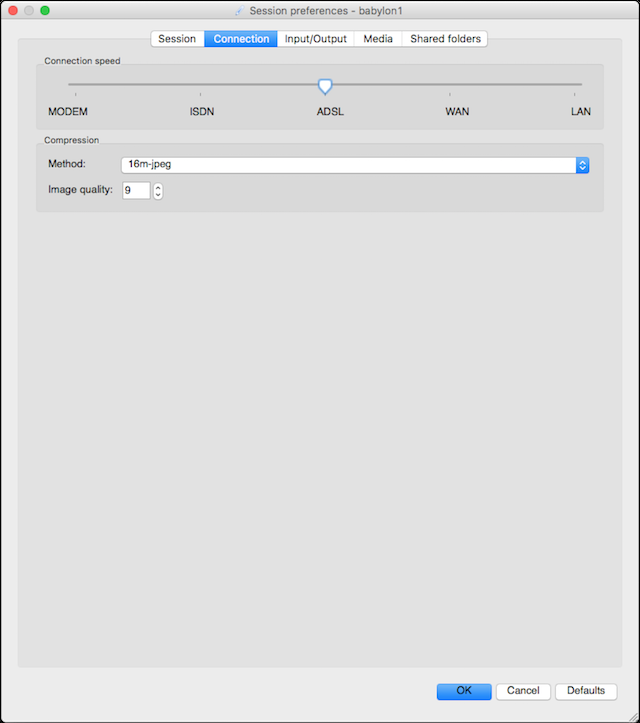
\includegraphics[width=6.4054in,height=5.31336in]{media/image2.png}

\textbf{Next Session:} Bubble Sort -- Simulations and Optimization

\textbf{Readings for the next session}: All the Chapters, especially 4
\& 8, ASIPMeister Tutorial \& Manual

\hypertarget{bubble-sort-simulation-optimisation}{%
\section{\texorpdfstring{\textbf{Bubble Sort --} Simulation \textbf{\&
Optimisation}}{Bubble Sort -- Simulation \& Optimisation}}\label{bubble-sort-simulation-optimisation}}

\textbf{{1 Week}}

\textbf{Motivation and introduction}

In this session, we will start applying the whole design flow to a
\emph{BubbleSort} algorithm. You will receive the C code for
\emph{BubbleSort} to be simulated. Afterwards you will optimize its
performance by adding new instruction(s). In a later session, we will
estimate what we have paid for this speedup; in terms of chip area,
power and energy consumption, i.e. we will compare the basis processor
with the modified/extended one. Finally, in a later session, we will
implement both processors on the FPGA board. For every part, that starts
like ``a)'', ``b)'' \ldots{} you have to mail the answers and asked
files to \textbf{sajjad.hussain@kit.edu} and use the topic
``asipXX-Session5'', with XX replaced by your group number.

\textbf{Exercices}

\begin{enumerate}
\def\labelenumi{\arabic{enumi}.}
\item
  \textbf{BubbleSort Algorithm}

  \begin{enumerate}
  \def\labelenumii{\arabic{enumii}.}
  \item
    Have a look at ``\emph{BubbleSort\_Index.c''}. Every part, which
    contains a \emph{printf} function call, is encapsulated with a
    \emph{``\#ifndef ASIP''} directive. The reason is, that the
    \emph{printf} function usually is resolved to an operating system
    call (managing the screen and other resources), but for our CPU we
    don't have an operating system, thus we ignore the \emph{printf}
    function for our simulations. For hardware execution in a later
    session, we will map this call to a UART terminal or LCD. For a
    \emph{gcc} compiled version the \emph{printf} is a helpful in
    debugging the output.
  \item
    Look at the implementation of the algorithm. You will need a good
    knowledge of the algorithm for later optimizations. Compile
    \emph{``BubbleSort\_Index.c''} with ``\emph{gcc BubbleSort\_Index.c
    --o BubbleSort\_Index}'', look at the printed output when executing
    the binary and understand how the algorithm is working by going
    through the printed output gradually.
  \end{enumerate}
\end{enumerate}

\begin{enumerate}
\def\labelenumi{\alph{enumi})}
\item
  How often the code of the inner loop is executed (not only the
  exchange part, the whole inner loop)? Please do not only answer this
  question, but also go through the output step by step. First, you
  should look at the code and think about the answer and then you should
  add a counter to the code to compute the correct result just to make
  sure, your prediction is correct.

  \begin{enumerate}
  \def\labelenumii{\arabic{enumii}.}
  \item
    To simulate \emph{BubbleSort} with \emph{dlxsim} and \emph{ModelSim}
    it has to be translated from C to assembly, which will be done in
    the later exercises. To make the translation easier, the
    ``\emph{BubbleSort\_Address.c''} has been prepared. Compile
    ``\emph{BubbleSort\_Address.c''} with \emph{gcc} as discussed
    before.
  \item
    First, make sure that the output of the \emph{gcc} compiled versions
    of ``\emph{BubbleSort\_Index.c''} and
    ``\emph{BubbleSort\_Address.c''} is the same. Then have a more
    detailed look into the address-version. The main difference between
    both versions is the way of accessing the array. The index-version
    uses an indexed access (e.g. array {[}j+1{]}). This usually
    translates into a chain of assembly instructions. First, the real
    address has to be computed and then the value can be loaded. The
    real address is: ``starting address from array'' + ``size of one
    array entry'' * ``index (i.e. j+1)''. In the inner loop of
    \emph{BubbleSort} we traverse through the array linearly, so we do
    not have to compute the real address every time from the scratch,
    instead we can just update the last computed real address. Two other
    changes against the index-version are, that every memory access is
    explicitly written, like ``\emph{value\_j = *j;}'' and the number of
    memory accesses is optimized as compared to the index-version.
  \end{enumerate}
\end{enumerate}

\begin{enumerate}
\def\labelenumi{\alph{enumi})}
\item
  How many load- and how many store- instructions are executed for each
  inner loop (distinguish between when there is exchange and no
  exchange)? Compare the index-version against the address-version and
  mention the two main points, why the address-version needs less memory
  accesses.
\end{enumerate}

\begin{enumerate}
\def\labelenumi{\arabic{enumi}.}
\setcounter{enumi}{1}
\item
  \textbf{Preparing your project}

  \begin{enumerate}
  \def\labelenumii{\arabic{enumii}.}
  \item
    You can use the same project as in the first session, and just
    create a separate application subdirectory for each example. You can
    start a fresh project as in the Session 1, but this would be time
    consuming.
  \item
    For the C application, you have to create subdirectory in the
    ``\emph{Application}'' directory (e.g. ``sorting''), and copy your
    application from ``\emph{/home/asip00/Sessions/Session6/bubble.c}''
    to here.
  \item
    Copy a ``\emph{Makefile}'' file from the ``\emph{TestPrint}''
    application subdirectory to each application subdirectory.
  \item
    Set proper parameters and settings in ``\emph{env\_settings}.
  \item
    For these exercises, we will be using pipeline forwarding (-pf1)
    option which is the default one.
  \item
    Make sure that you already have VHDL files and GNU tools in your
    project's meister directory.
  \end{enumerate}
\item
  \textbf{Compiling the application in dlxsim and ModelSim with basis
  processor}

  \begin{enumerate}
  \def\labelenumii{\arabic{enumii}.}
  \item
    Now, compile ``bubble.c'' using ``make sim''.
  \item
    After compiling, simulate the application in \emph{dlxsim} and
    \emph{ModelSim} and compare whether the printed results are the same
    compared to a \emph{gcc}-compiled version. For dlxsim, you can use
    the command ``get \_array 20d'', it should give you the sorted
    array. For ModelSim, you can see the sorted array in the
    TestData.OUT file.
  \end{enumerate}
\end{enumerate}

\begin{enumerate}
\def\labelenumi{\alph{enumi})}
\item
  How many cycles do you need for execution in dlxsim and ModelSim?
\end{enumerate}

\begin{enumerate}
\def\labelenumi{\arabic{enumi}.}
\setcounter{enumi}{3}
\item
  \textbf{Bubble Sort -- Optimisation: Customizing the basis processor}

  \begin{enumerate}
  \def\labelenumii{\arabic{enumii}.}
  \item
    Create a project directory for this session by copying the directory
    ``\emph{/home/asip00/­epp/ASIP­Meister­Projects/TEMPLATE\_PROJECT/}''
    and renaming it (e.g. \emph{brownieOPT}).
  \item
    Now we start optimizing our bubblesort application for speed. There
    might be two options for you.

    \begin{enumerate}
    \def\labelenumiii{\arabic{enumiii}.}
    \item
      Create a new application sub-directory (e.g. ``sortingOptS'') and
      copy ``sorting/BUILD\_SIM/bubble.s'' from the last exercise to
      this directory and start optimizing the code. In the assembly
      code, look for different possibility to define custom instructions
      and replace that part of code with the custom instruction in
      assemble file. If you start with assembly file, sometime it gives
      errors for labels that starts with dot. Change it to dashes. like
      .L6 to \_L6.
    \item
      Create a new application sub-directory (e.g. ``sortingOptC'') and
      copy ``bubble.c'' to this directory and start optimizing the code.
      You can directly look into the ``bubble\emph{.c}'' and define some
      custom instruction to replace some part of the code with new
      custom instruction.
    \end{enumerate}
  \item
    However, before optimizing, create a simple C or assembly file to
    test different custom instruction (e.g. OPT) into an application
    subdirectory i.e. \emph{TestOPT}.
  \item
    Copy a ``\emph{Makefile}'' file from the ``\emph{TestPrint}''
    application subdirectory to each application subdirectory.
  \item
    Copy the provided \emph{ASIPMeister} CPU file
    ``\emph{browstd32.pdb''} from ``/home/asip00//Sessions/Session1/''
    into your project directory, and rename it
    ``\emph{browstd32OPT.pdb''}
  \item
    Set proper parameters and settings in ``\emph{env\_settings}'' as
    discussed in Figure 2-5 in the Laboratory Script. Specially the
    followings:
  \end{enumerate}
\end{enumerate}

\begin{quote}
export PROJECT\_NAME=brownieOPT

export CPU\_NAME=browstd32OPT

export ASIPMEISTER\_PROJECTS\_DIR=\$\{HOME\}/ASIPMeisterProjects

export DLXSIM\_DIR=/home/asip00/epp/dlxsimbr\_Laboratory
\end{quote}

\begin{enumerate}
\def\labelenumi{\arabic{enumi}.}
\setcounter{enumi}{4}
\item
  \textbf{Adding the new instruction to \emph{ASIPMeister}}

  \begin{enumerate}
  \def\labelenumii{\arabic{enumii}.}
  \item
    Now we start adding new instructions to our processor to speed up
    the execution.
  \item
    In your project directory start \emph{ASIPMeister} and add the new
    instruction to your new CPU. First, define a new instruction format
    for your instruction if it does not match with the existing
    instruction formats.
  \item
    Use the available opcode.
  \end{enumerate}
\end{enumerate}

\begin{enumerate}
\def\labelenumi{\arabic{enumi}.}
\item
  You also have to define ``CKF Prototype'' for each new custom
  instruction in ASIPmeister, generate GNU tools and use inline assembly
  in C code.

  \begin{enumerate}
  \def\labelenumii{\arabic{enumii}.}
  \item
    Add the custom instructions to dlxsim as well.
  \item
    Write a small C or assembly code to test your new instruction.
  \item
    Generate the hardware and software files from ASIPMeister and
    simulate the new instruction with \emph{ModelSim}. Use the small
    test application that you created to test your \emph{dlxsim}
    implementation in the previous exercises for this purpose.
  \item
    If everything is working fine, then simulate the \emph{BubbleSort}
    C/Assembly code that uses the new instruction in \emph{ModelSim}.
  \item
    Compile the optimized bubblesort application using ``\emph{make
    sim}'' and then ``\emph{make dlxsim}''. Make sure, that the
    resulting array is still correct.
  \end{enumerate}
\end{enumerate}

\begin{enumerate}
\def\labelenumi{\alph{enumi})}
\item
  How many cycles do you need for execution?
\item
  What is the speedup compared to \emph{original code} (i.e. \#Cycles
  without custom instruction / \#Cycles with custom instruction)?
\item
  Attach the assembly and/or C file you used to test the custom
  instruction and to test the given application.
\item
  Attach the modified ASIPmeister .pdb file.
\end{enumerate}

\textbf{Next Session:} Bubble Sort - \textbf{Power \&} Area
\textbf{Estimation and} Hardware Implementation

\textbf{Readings for the next session}: Laboratory Chapters 6 \& 7

\hypertarget{bubble-sort-power-area-estimation-and-hardware-implementation}{%
\section{\texorpdfstring{\textbf{Bubble Sort -- Power \&} Area
\textbf{Estimation and Hardware
Implementation}}{Bubble Sort -- Power \& Area Estimation and Hardware Implementation}}\label{bubble-sort-power-area-estimation-and-hardware-implementation}}

\textbf{{1 Week}}

\textbf{Motivation and introduction}

In this exercise, you will synthesize and implement the bubblesort
application and then download it to FPGA board and see the results on
the UART terminal or LCD. For visualizing, the output of BubbleSort and
some additional information is printed to the URAT interface. You can
use t\_print() for directing output to LCD or u\_print() to UART.
Remember, you need to add respective libraries. Using these frameworks,
the Bubble sort algorithm which will be implemented using the two CPUs
to form two versions:

\textbf{Version1:} basis CPU (\emph{browstd32.pdb})

\textbf{Version2:} optimized CPU (\emph{browstd32opt.pdb}) which
supports new instructions

For every part, that starts like ``a)'', ``b)'' \ldots{} you have to
mail the answers and asked files to \textbf{sajjad.hussain@kit.edu} and
use the topic ``asipXX-Session6'', with XX replaced by your group
number.

\textbf{Exercises}

\begin{enumerate}
\def\labelenumi{\arabic{enumi}.}
\item
  \textbf{Preparing and Simulating Version 1}

  \begin{enumerate}
  \def\labelenumii{\arabic{enumii}.}
  \item
    You have to create the software and the hardware sub directories
    under ``\emph{Application}'' for browstd32.pdb CPU. First, create a
    new project directory inside your \emph{ASIPMeisterProjects}
    directory for the new CPU and name it ``\emph{browstd32''}. You can
    use a copy from the \emph{browstd32} CPU project from the last
    session, but do not forget to adjust the ``\emph{env\_settings''}.
    Remember, for LCD interface you need to create two separate
    subdirectories for the software and the hardware application in
    ``Applications'' directory.
  \item
    Copy the provided and ``\emph{app\_UART.c''} from
    ``/home/asip00/Sessions/Session7'' to the created LCD or UART
    subdirectories respectively. This file directs the printing to UART,
    you can change it to LCD by replacing u\_print() to t\_print().
    However, UART interfacing is sufficient.
  \item
    Copy the C libraries from ``\emph{asip00/epp/StdLib}'' to each
    application subdirectory. For LCD simulation in dlxsim and ModelSim,
    use ``lib\_lcd\_dlxim.c''. For real LCD implementation in FPGA use
    ``lib\_lcd\_320.c''.
  \item
    Also, copy the ``\emph{Makefile}'' to both the subdirectories.
  \item
    Make sure that you already have generated the VHDL files and GNU
    Tools for your CPU.
  \item
    Compile (``\emph{make sim}'') the application for basis CPU and
    generates the required .dlxsim and DM/IM file for the dlxsim and
    ModelSim respectively.
  \item
    Simulate the application with dlxsim using ``\emph{make dlxsim
    DLXSIM\_PARAM=''-da0 --pf1 --ufBubbleUART.out''}''. It will start
    the dlx simulator to simulate the compiled file generated in the
    previous stage. Here, you have to pass some parameters to dlxsim
    such as the LCD/UART file to print the outputs.
  \item
    You can restart the CPU by pressing the ``\emph{reset}'' push button
    on the small mini board on the FPGA board, but REMEMBER, that your
    array in data memory is already sorted after the first run, so the
    second, third \ldots{} run will be significantly faster than the
    first one.
  \item
    The BubbleSort framework is measuring the number of cycles for the
    execution of the bubbleSort methods. This measurement is done by a
    counter on the FPGA Board or in dlxsim/ModelSim respectively. This
    measurement only measures the bubbleSort method, but not the
    overhead for e.g. printing the result.
  \end{enumerate}
\item
  \textbf{Implementing the Project}

  \begin{enumerate}
  \def\labelenumii{\arabic{enumii}.}
  \item
    Create your ISE project as discussed in the session 4. Synthesize,
    implement and generate the bitfiles.
  \item
    Then from the application direcotory run ``make fpga'' and ``make
    upload''.
  \item
    You can check the results on the UART. You can open HyperTerminal
    using ``hterm \&''.
  \end{enumerate}
\end{enumerate}

\begin{enumerate}
\def\labelenumi{\alph{enumi})}
\item
  If your design works correctly, find out the design statistics
  (critical path, maximum frequency and area)
\item
  Compute the accurate time (in ms) required to sort the 20 numbers. Use
  the number of executed cycles (printed on the URAT interface) and the
  max. CPU frequency on the FPGA board, where the sorting is still
  correct).
\item
  Analyse the time and find the critical path (see Chapter 6.5 of the
  Laboratory Script)
\end{enumerate}

\begin{enumerate}
\def\labelenumi{\arabic{enumi}.}
\setcounter{enumi}{2}
\item
  \textbf{Power Estimation}

  \begin{enumerate}
  \def\labelenumii{\arabic{enumii}.}
  \item
    During ModelSim simulation also generate the VCD files for mentioned
    frequencies (first with 50MHz and then with Max. Frequency found in
    the last session).
  \item
    Create Xilinx ISE project to estimate power with XPower.
  \end{enumerate}
\end{enumerate}

\begin{enumerate}
\def\labelenumi{\alph{enumi})}
\item
  Determine the total and dynamic power.
\item
  Compute the total execution time (ms). You can use execution as the \#
  of cycles multiplied by the clock cycle in ModelSim.
\item
  Compute the energy required. Fill in all these results in the table
  below e.g. \emph{PowerReport.xlx} or \emph{PowerReport.ods}.
\item
  Does using any instruction minimize the required energy? A version
  uses an application, which needs less number of clock cycles than
  another Version; is it also power and/or energy-optimized version
  compared to Version2?
\item
  Repeat a-d, but instead of taking the default of 50 MHz, use the
  individual maximum CPU frequency on which a CPU can run (You can get
  it from ISE\_Benchmark). This frequency has to be configured in
  tb\_brownie32std.vhd (search for CLK\_PERIOD; e.g. 10 ns half period =
  20 ns period = 50 MHz). XPower will automatically load this frequency
  from the VCD file.
\end{enumerate}

\begin{enumerate}
\def\labelenumi{\arabic{enumi}.}
\setcounter{enumi}{3}
\item
  \textbf{Preparing, Simulating, Implementing and Power Estimation for
  Version2}

  \begin{enumerate}
  \def\labelenumii{\arabic{enumii}.}
  \item
    Repeat the above exercises for the optimized version a), b), c), d),
    e).
  \item
    Sample PowerReport.xlx or PowerReport.ods
  \end{enumerate}
\end{enumerate}

\begin{longtable}[]{@{}lllll@{}}
\toprule
\endhead
& Total Power {[}mW{]} & Dynamic Power {[}mW{]} & Execution Time
{[}ms{]} & Energy {[}nJ{]}\tabularnewline
\textbf{Version1} 50 MHz & & & &\tabularnewline
\textbf{Version2} 50 MHz & & & &\tabularnewline
\begin{minipage}[t]{0.17\columnwidth}\raggedright
\textbf{Version1}

Max. Freq: -\/-\/-\/-\/-MHz\strut
\end{minipage} & \begin{minipage}[t]{0.17\columnwidth}\raggedright
\strut
\end{minipage} & \begin{minipage}[t]{0.17\columnwidth}\raggedright
\strut
\end{minipage} & \begin{minipage}[t]{0.17\columnwidth}\raggedright
\strut
\end{minipage} & \begin{minipage}[t]{0.17\columnwidth}\raggedright
\strut
\end{minipage}\tabularnewline
\begin{minipage}[t]{0.17\columnwidth}\raggedright
\textbf{Version2}

Max. Freq: -\/-\/-\/-\/-MHz\strut
\end{minipage} & \begin{minipage}[t]{0.17\columnwidth}\raggedright
\strut
\end{minipage} & \begin{minipage}[t]{0.17\columnwidth}\raggedright
\strut
\end{minipage} & \begin{minipage}[t]{0.17\columnwidth}\raggedright
\strut
\end{minipage} & \begin{minipage}[t]{0.17\columnwidth}\raggedright
\strut
\end{minipage}\tabularnewline
\bottomrule
\end{longtable}

\textbf{Next Session:} Adaptive Differential Pulse Code Modulation
(ADPCM)

\textbf{Readings:} Recall relevant information from Laboratory Script,
ASIPmeister Tutorial and User Manual

\hypertarget{adaptive-differential-pulse-code-modulation-adpcm}{%
\section{\texorpdfstring{Adaptive \textbf{Differential Pulse Code
Modulation
(ADPCM)}}{Adaptive Differential Pulse Code Modulation (ADPCM)}}\label{adaptive-differential-pulse-code-modulation-adpcm}}

\textbf{{3 Weeks}}

\textbf{Motivation and introduction}

This is the final session. You have \textbf{{Three}} weeks to complete
this session, but you will need these weeks! In this exercise, you will
work with an IoT application for which you have to create an optimized
CPU. There are different possible ways to modify the CPU, depending on
your goals and the \textbf{{area/power}} that you want to spend for the
custom instructions. After the CPU has been modified, you will benchmark
it to get an idea, what you have to pay for your optimizations. In the
last semester week, you will present your results to other groups. The
presentations will take place in the Meeting Room 316.2, the exact date
and time will be decided mutually. For every part, that starts like
``a)'', ``b)'' \ldots{} you have to mail the answers and asked files
with a CC to your group members to \textbf{sajjad.hussain@kit.edu} and
use the topic ``asipXX-Session8'', with XX replaced by your group
number.

\textbf{Exercises}

\begin{enumerate}
\def\labelenumi{\arabic{enumi}.}
\item
  \textbf{The Application:}

  \begin{enumerate}
  \def\labelenumii{\arabic{enumii}.}
  \item
    The application is the ADPCM audio decoder.
  \item
    The term Pulse-Code Modulation (PCM) denotes uncompressed audio
    samples and Adaptive Differential Pulse-Code Modulation (ADPCM) use
    an adaptive prediction for the next audio sample with a lossy
    quantization (i.e. the audio signal will not be exactly the same
    after encoding and decoding).
  \item
    You can find the source code for ADPCM decoder with some ADPCM
    encoded audio data in /home/asip00/Sessions/Session8. When you run
    the ADPCM decoder, you can recover the original audio samples
    (approximately).
  \item
    Two different versions of the encoded audio data are provided,
    differing in the size of input data. The MINI version is meant for
    the initial tests, i.e. use it to test whether your application
    compiles and whether dlxsim and ModelSim can simulate it. However,
    the MINI version is too short to hear anything meaningful when
    playing it on the FPGA prototype board. The BRAM version is the
    biggest possible version that fits into the FPGA-internal memory
    (called Block RAM). While testing your application on FPGA you have
    to use this BRAM version. For dlxsim/ModelSim simulation comment the
    while(1) loop, while for FPGA implementation use while(1) loop
    without any print statement inside it.
  \item
    In our application, the uncompressed audio data has 16 Bits per
    sample. The ADPCM encoded audio data has 4 Bits per sample; two
    samples are stored together in one Byte.
  \item
    The provided encoded audio data is sampled with a certain frequency
    (i.e. samples per second = sample rate); in our case 96000 samples
    per second. ADPCM does not need this information; it simply looks at
    one sample after the other.
  \item
    You can change the CPU frequency by using the knob existed on the
    small extra PCB which is connected to the FPGA board. Here, you can
    find a table describing knop position and corresponding frequencies.
  \item
    Changing the frequency, you can figure out what is the slowest
    possible frequency that makes the CPU decode correctly the audio
    samples (i.e. the sound still hearable enough without corruption).
  \end{enumerate}
\end{enumerate}

\begin{longtable}[]{@{}ll@{}}
\toprule
Knob value & Frequency (MHz)\tabularnewline
\midrule
\endhead
0 & 100\tabularnewline
1 & 80\tabularnewline
2 & 66\tabularnewline
3 & 50\tabularnewline
4 & 40\tabularnewline
5 & 25\tabularnewline
Else & 100\tabularnewline
\bottomrule
\end{longtable}

Table-1: Frequency Changing

\begin{enumerate}
\def\labelenumi{\arabic{enumi}.}
\setcounter{enumi}{1}
\item
  \textbf{Your Tasks}
\end{enumerate}

You have to perform the following tasks, the details for which are given
in the following exercises.

\begin{enumerate}
\def\labelenumi{\arabic{enumi}.}
\item
  To make your optimization comparable with other groups start with the
  browstd32 CPU provided in Session 1, and test ADPCM application. {Do
  not take any CPU that you already have modified}).
\item
  Compile the MINI version of the application; simulate it with
  dlxsim/ModelSim.
\item
  Then compile the BRAM version and run it on the FPGA prototype.
\item
  Which frequency do you need until the decoding is fast enough? You can
  hear the difference when gradually increasing the frequency. When
  there is no difference from one frequency to the other, then the
  slower one was fast enough.
\item
  Improve/Extend the CPU for speed, power or area. You have to create
  two different versions based on your improvements. You should have at
  least two extensions (power, performance or area).
\item
  Test the improved CPU version on dlxsim/ModelSim and on FPGA
\item
  Benchmark the basis and improved CPUs for area, frequency, power,
  execution time etc.
\item
  Prepare slides that explain your modifications, improvements and
  results to compete with other groups.
\item
  Typically, we will not simulate in dlxsim but mainly in ModelSim. For
  the extended CPUs you have to generate new compiler as we did in the
  previous sessions.
\end{enumerate}

\begin{enumerate}
\def\labelenumi{\arabic{enumi}.}
\setcounter{enumi}{2}
\item
  \textbf{Simulating the Application}

  \begin{enumerate}
  \def\labelenumii{\arabic{enumii}.}
  \item
    Prepare your new project directory and create a subdirectory in your
    ``\emph{Applications}'' directory and copy
    ``\emph{/home/asip00/Sessions/Session8/adpcm.c}'' to this
    subdirectory. Also, copy the required ``\emph{Makefile}''.
  \item
    To compile the application, audio data is needed for decoding;
    therefore, you have to copy the audio data that shall be used for
    decoding. Two different-sized versions of the same audio stream are
    provided in ``\emph{/home/asip00/Sessions/Session8/}''. To copy the
    required audio data \emph{adpcmDataStereo\_MINI.h or
    adpcmDataStereo\_BRAM.h} into subdirectory as \emph{adpcmData.h}.
    The compilation will take some time due to the large audio data. For
    short tests, e.g. to test whether the inline assembly code compiles
    and assembles or whether ModelSim simulation gives the correct
    output, use the ``\emph{adpcmDataStereo\_MINI.h}'' version of the
    file.
  \item
    Copy dlxsim simulator to your home directory to implement new custom
    instruction here. Set ``\emph{env\_settings}'' accordingly. Usually
    it is sufficient to simulate the application with ModelSim, but you
    can also simulate it with dlxsim.
  \item
    First you have to compile the application using gcc compiler to
    compare with the later results from dlxsim and ModelSim, forward the
    gcc printed output to a file, e.g. ``\emph{a.out \textgreater{}
    output\_gcc.txt}''.
  \item
    Copy the required libraries from \emph{``/home/asip00/epp/StdLib}''
    to the application subdirectory and compile ADPCM application using
    ``make sim''.
  \item
    After compiling, simulate the application in \emph{dlxsim} and
    \emph{ModelSim} and compare whether the printed results are the same
    compared to a \emph{gcc}-compiled version. The \emph{gcc} version
    will print the arrays on the screen and \emph{dlxsim} and
    \emph{ModelSim} will print them to a \emph{virtual} LCD. For
    \emph{dlxsim} you can forward the LCD output to a file, using the
    ``-lf'' parameter or forward the audio channel data to a file using
    ``\emph{-af}'' parameter. \emph{ModelSim} automatically writes LCD
    output to the file `lcd.out' and audio channel data to ``audio.out''
    The application can write the decoded audio data to the audio output
    (to hear it) or it can write the data to the LCD/UART (to see it).
    You can define this behavior with the ``\emph{\#define
    PRINT\_ARRAY}'' switch, when set to 1 the decoded hexadecimal data
    is print in ModelSim generated ``\emph{lcd.out}'' and in a file
    generated with --lf option in dlxsim. When ``\emph{PRINT\_ARRAY}''
    is set to 0, decode data for left/right channel is saved in ModelSim
    generated audio.out and in a file generate with ``\emph{--af}''
    option in dlxsim. ModelSim will create an `audio.out' file and
    dlxsim will write the data to screen (unless you use the
    ``\emph{-af\{filename\}}'' parameter then it will write it to file).
  \item
    Save the printed results from the ModelSim simulation of the
    original CPU. Then you can compare them with the printed results
    from your modified CPU; they have to be identical!
  \end{enumerate}
\item
  \textbf{Running the Application on FPGA}

  \begin{enumerate}
  \def\labelenumii{\arabic{enumii}.}
  \item
    To test whether the decoder is working correct with the base CPU and
    later with your modified CPU, you have to run the application on the
    FPGA prototype (test it with ModelSim first).
  \item
    We have a simple digital- analog converter (DAC) periphery. This DAC
    is memory mapped attached to the CPU, i.e. the applications `saves'
    the decoded audio values to a certain address. The methods
    ``\emph{writeToAudioOutR(int data)}'' and
    ``\emph{writeToAudioOutL(int data)}'' are provided in the
    \emph{lib\_audio} library.
  \item
    The hardware will automatically send the audio samples with a
    certain sample rate to the audio out pin. The sample rate of the
    hardware has to match the sample rate of the audio data; otherwise,
    the audio will play too fast or too slow. The sample rate of the
    hardware can be configured in the file ``\emph{dlx\_Toplevel.vhd}''
    i.e. ``\emph{KSAMPLES\_PER\_SECOND}'' should be set to 96). This is
    the correct sample rate for the provided audio data.
  \item
    Whenever you write audio data to the hardware audio out it will be
    buffered in a FIFO. The data of this FIFO is automatically read with
    the (above-mentioned) sample rate. You may write to this FIFO as
    fast as you can compute the data. However, if the FIFO is full, then
    the store instruction ``sw'' will stall until some space becomes
    free.

    \begin{enumerate}
    \def\labelenumiii{\arabic{enumiii}.}
    \item
      Therefore, if your application executes faster than this FIFO is
      read, then the FIFO will slow down your execution. This gives you
      the possibility to slow down the clock to save energy, or to run
      other tasks in the case of a multi-tasking environment.
    \item
      If your application runs too slow, then the FIFO will become
      empty, resulting in errors in the audio stream. Try it!
    \item
      These effects do not appear in \emph{dlxsim} or \emph{ModelSim}
      simulation, as they do not model/simulate the FIFO, but just
      perform a simple ``\emph{sw}'' operation.
    \end{enumerate}
  \end{enumerate}
\item
  \textbf{Extending the Basis CPU}

  \begin{enumerate}
  \def\labelenumii{\arabic{enumii}.}
  \item
    You may add new custom instructions to speed up frequent
    computations in adpcm.c. If your custom instruction delays to clock
    too much, then you can change it into a multi-cycle instruction
    (i.e. an instruction that is allowed to stay in EXE stage for
    multiple cycles, similar to ``mult''). The details about multi-cycle
    FHM are given in Chapter 4.4 of the Laboratory Script.
  \item
    You may change parameters for existing hardware blocks. One typical
    example is the number of read/write ports of the register file,
    depending on the requirements of your custom instructions.
  \item
    It is complicated (but possible) to change the number of registers
    in the register file. To do this, all instruction formats have to be
    modified. If you for example, only use 16 registers, then you only
    need 4 bits in the 32-bit instruction to denote which register you
    want to access. Therefore, you have to adapt the instruction formats
    such that only 4 bits are used to address the register (simplest way
    is to make one of the bits a constant `0' in the instruction
    format). Additionally, you have to modify the assembly code (or
    directly the compiler, but changing the assembly code seems simpler)
    to make sure that only the lower 16 registers are used. Creating a
    compiler with 16 register is still possible, but needs some
    debugging.
  \item
    {\textbf{You have to create, test, and benchmark TWO}
    \textbf{different} \textbf{CPUs with different optimizations}}. For
    example, you might create one CPU that is optimized for performance
    considering the cycles in ModelSim or the CPU that is optimized for
    the power/energy due to a reduced clock frequency that is possible
    due to a faster computation or the CPU that is optimized for area,
    e.g. by removing not required instructions/hardware blocks etc.
  \end{enumerate}

  \begin{enumerate}
  \def\labelenumii{\alph{enumii}.}
  \item
    Attach to mail your both ASIPMeister CPU optimized for
    area/performance/power named like ``\emph{browstd32Area.pdb}'',
    ``\emph{browstd32Power.pdb}'' or ``\emph{browstd32Speed.pdb}'' etc.
  \item
    Attach to mail if you have defined new hardware resources (.fhm
    files) in ASIPMeister.
  \item
    Attach with the mail your adpcm.c, which you modified with your
    custom instructions, for the two CPU optimizations.
  \item
    Attach the test application files that you created to test new
    instructions.
  \end{enumerate}
\item
  \textbf{Benchmarking the CPUs}

  \begin{enumerate}
  \def\labelenumii{\arabic{enumii}.}
  \item
    \textbf{Make benchmarks for the old (\emph{browstd32}) and the two
    modified CPUs and compare them with each other. For the benchmarking
    you have to take care of the following points:}

    \begin{enumerate}
    \def\labelenumiii{\arabic{enumiii}.}
    \item
      \textbf{Make sure, that you do all benchmarks very accurate to
      make them comparable!}
    \item
      \textbf{Always use MINI version of the application}
    \item
      \textbf{Always compile with ``-O3'' to achieve the best compiler
      output. Note: For debugging purpose ``-O0'' (default) is
      recommended.}
    \item
      \textbf{Always using ISE\_Benchmark framework for the area, power
      and critical path analysis}
    \item
      \textbf{Always take execution time or number of cycles from
      ModelSim}
    \item
      \textbf{For execution time, power, and energy use the following
      three CPU frequencies:}

      \begin{enumerate}
      \def\labelenumiv{\arabic{enumiv}.}
      \item
        \textbf{50 MHz; to make it comparable among the groups}
      \item
        \textbf{The slowest frequency that is sufficient to execute the
        application fast enough; to see the lowest power consumption. To
        calculate the slowest still fast enough frequency you have to
        consider the number of cycles that your application requires to
        execute the decoder and the time-budget that you have for
        decoding. The time-budget depends on the number of audio samples
        and the sample-rate. The sample-rate is configured to 96000
        Samples per second. The number of samples depends to the number
        of entries in your audio-data array. Remember, that -- in the
        compressed array -- each sample just requires 4 Bit.}
      \item
        \textbf{The fastest frequency that your CPU supports (given by
        ISE\_Benchmark framework); to see the peak performance}
      \end{enumerate}
    \item
      \textbf{You have to configure the frequency in the ModelSim
      testbench for power estimation. Remember that you have to
      configure the half clock period.}
    \end{enumerate}
  \item
    \textbf{You have to benchmark and compare the following points:}

    \begin{enumerate}
    \def\labelenumiii{\arabic{enumiii}.}
    \item
      \textbf{CPU Area}
    \item
      \textbf{Maximal CPU frequency or Critical Path}
    \item
      \textbf{Number of Cycles or Execution Time}
    \item
      \textbf{Dynamic Power Consumption}
    \item
      \textbf{Energy Consumption}
    \end{enumerate}
  \end{enumerate}
\item
  \textbf{Presenting the Results}

  \begin{enumerate}
  \def\labelenumii{\arabic{enumii}.}
  \item
    \textbf{In} the last week of the semester, you have to present your
    results to the other groups. Therefore, every group has to prepare
    slides to:
  \item
    \textbf{Explain the two different CPUs that you have created to
    optimize ADPCM application.}
  \item
    \textbf{Present the problems that you faced while implementing the
    two new CPUs. This is the interesting part! Maybe also talk about
    some implementations that you thought about but which you did not
    realize.}
  \item
    \textbf{Discuss your benchmark results; for every point you should
    have one slide on which the results are shown in a graph (bar graph,
    lines \ldots).}
  \item
    \textbf{Print proper units your axes e.g. ``Execution time
    {[}s{]}'', ``Execution time {[}cycles{]}'', ``Power consumption
    {[}mW{]}'', \ldots).}
  \item
    \textbf{For every} measurement point, print the value of this
    measurement result to make comparisons easier.
  \end{enumerate}
\end{enumerate}

\begin{enumerate}
\def\labelenumi{\alph{enumi})}
\item
  You have to mail the slides before the presentation. Name the slides
  like ``asipXX\_presentation.ppt'' (or ``.odp'' or ``.pdf'').
\item
  You have to explain which benchmarks you used while customizing the
  processor and compare in the presentation.
\end{enumerate}

\end{document}
